\chapter{Simulador Metagenómico PyMetaSeem}
Un problema abierto en la metagenómica es distinguir la calidad del ensamblaje y la correcta asignación taxonómica de los datos metagenómicos. Para lo cual es necesario tener datos metagenomicos de referencia de calidad, que contengan un sistema de clasificacion de la calidad de estos datos debidamente clasificados taxonomicamente, y de alta calidad para poder realizar la evaluacion de las herramientas de software de clasificación taxonomica y  de ensamblaje. Por esto se han realizado distintos simuladores de datos metagenomicos, los cuales se revisan en este capitulo, llegando a la conclusión de que la gran mayoria tienen complicaciones para su uso, y asi empezaremoscon la creaccion de nuestro propio simulador de datos metagenomicos.   \\

%\begin{figure}[h]
%\centering
%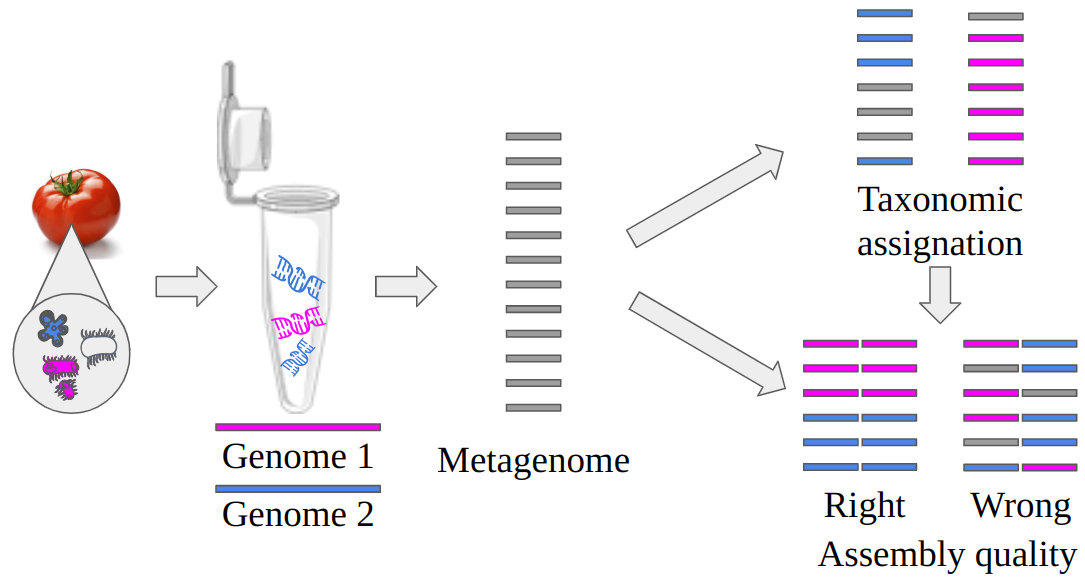
\includegraphics[width=\textwidth]{Img/cap2/problem.png}
%\caption{Flujo }
%\end{figure}


\section{PyMetaSeem: simulador de datos metagenómicos a partir de un conjunto de datos genómicos}

PyMetaSeem es un algoritmo creado desde cero que simula datos metagenómicos a partir de datos genómicos. Este simulador de datos metagenómicos fue creado a partir de reads recortadas de datos genómicos. Los genomas reales se utilizan para calificar la precisión de los clasificadores y ensambladores taxonómicos. Está pensado como un entorno conda, escalable, reproducible, fácil de usar y gratuito para el público ya que otros simuladores conocidos (como CAMISIM) tienen dificultades de instalación e implementación.  \\


%\begin{figure}[h]
%\centering
%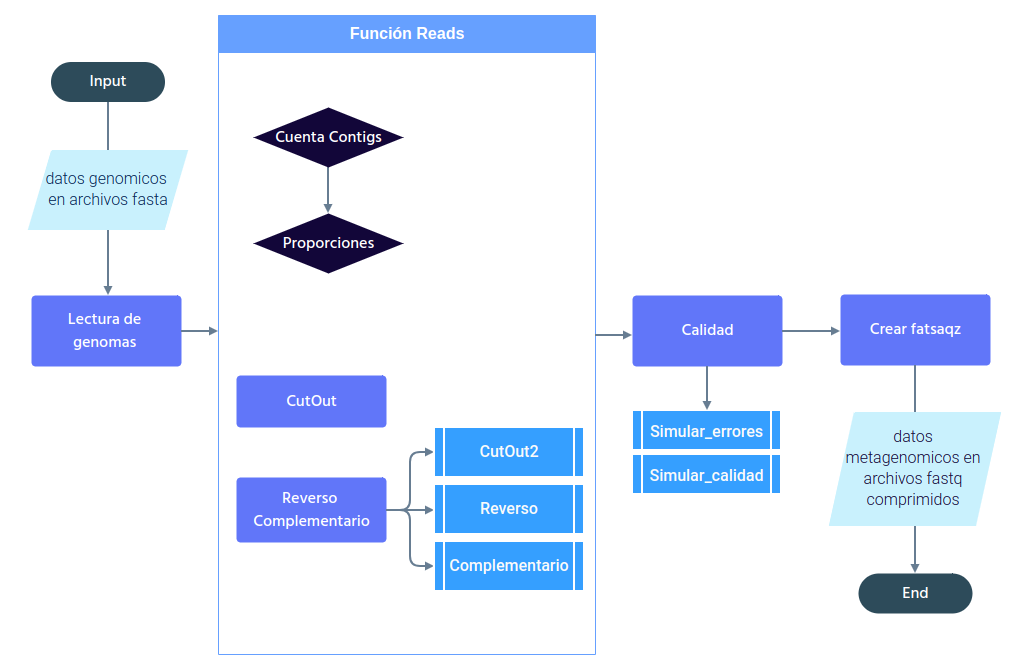
\includegraphics[width=\textwidth]{Img/cap2/diagrams_de_flujo.png}
%\caption{Diagrama de Flujo PyMetaSeem}
%\end{figure}

Este algoritmo está compuesto de varias funciones:

PyMetaSeem recibe un conjunto de archivos con diferentes genomas en formato FASTA, para esto se tienen las opciones de inicializar el algoritmo con numero de reads y longitud de reads ya sea manual o en un archivo de texto (txt) que contenga elnombre de los archivos y la cantidad de reads por genoma (perfil taxonomico).  \\

Se tiene una función que se encarga de de la lectura de los fasta, convirtiendolos en un diccionario que contiene cada secuencia de nucleótidos como valor y su nombre o identificador como clave, lo que facilita la gestión de los datos dentro de python.   \\

Teniendo los genomas en diccionarios, se crean varias funciones para tomar las longitudes de los reads a recortar y las proporciones,  tomando en cuenta el tamaño original de los contigs. Luego de obtener las longitudes y proporciones, se cortan los reads aleatorias (m) de una longitud determinada (n) a partir de la secuencia de nucleótidos.  \\


\subsection{Simulaciones}

%\begin{figure}[h]
%\centering
%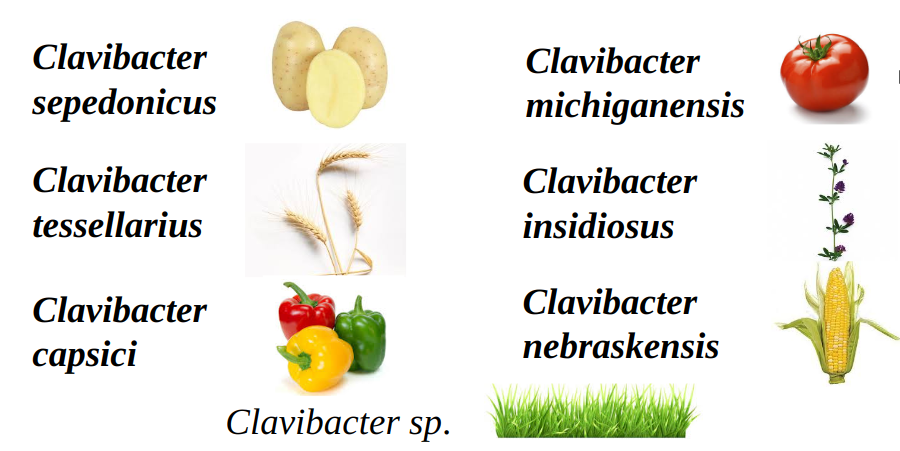
\includegraphics[width=\textwidth]{Img/cap2/clavibacter.png}
%\caption{Clavibacter}
%\end{figure}

\subsection{Comparaciones}


\section{Comparación taxonomica}

\section{Generalizando el N50, nuevas métricas para ensamblados de metagenoma}

En cuanto a la calidad de los ensamblajes, evaluamos la pertinencia de aplicar la métrica genómica N50 a los datos metagenómicos.  \\
(Videvall, 2017)  \\

Se trata de una medida utilizada para evaluar la contigüidad y la calidad del ensamblaje de un genoma. Los contigs de un ensamblaje se ordenan por tamaño y se suman, empezando por el mayor. Se toma el tamaño del contig que hace que el total sea mayor o igual al 50\% del tamaño del genoma.  \\


%\begin{figure}[h]
%\centering
%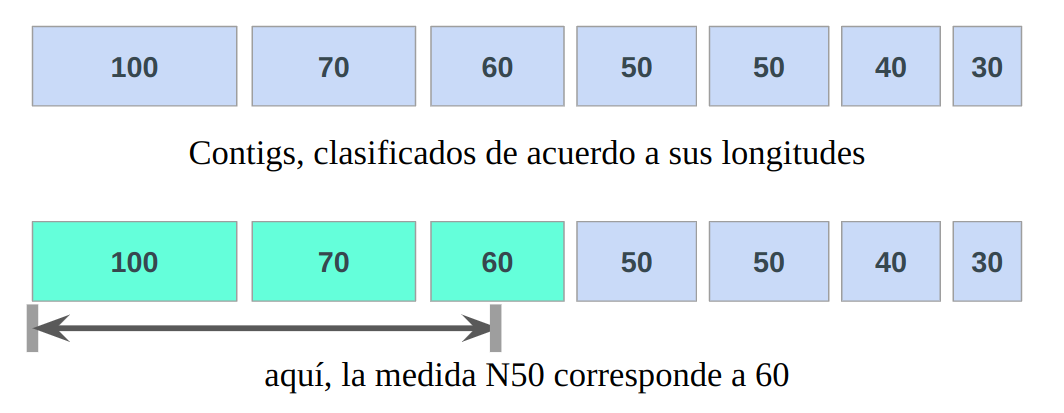
\includegraphics[width=\textwidth]{Img/cap2/N50_es.png}
%\caption{N50 }
%\end{figure}

N50 es una medida de calidad de secuencias genómicas (Miller et al., 2010; Videvall, 2017) (“metagenómica”), la cual se mide ordenando la totalidad de las secuencias de mayor a menor longitud, y sumando todas las longitudes hasta llegar al 50\% del total de la suma; la longitud de la secuencia que esté en este 50\% será la medida N50.  \\

Una medida típica para evaluar el éxito del ensamblaje es la medida N50, que equivale a la longitud del scaffold (o contig) que se solapa con el punto medio de la concatenación de scaffolds (contigs) por orden de longitud. Mäkinen, V., Salmela, L. \& Ylinen, J. Métrica de ensamblaje N50 normalizada mediante encadenamiento colineal restringido por espacios. BMC Bioinformática 13 , 255 (2012). https://doi.org/10.1186/1471-2105-13-255   \\

L50 es una medida de calidad de secuencias genómicas\\
